
\let\negmedspace\undefined
\let\negthickspace\undefined
\documentclass[article]{IEEEtran}
       \def\inputGnumericTable{}                                 %%
\usepackage{cite}
\usepackage{amsmath,amssymb,amsfonts,amsthm}
\usepackage{algorithmic}
\usepackage{graphicx}
\usepackage{textcomp}
\usepackage{xcolor}
\usepackage{txfonts}
\usepackage{listings}
\usepackage{enumitem}
\usepackage{mathtools}
\usepackage{gensymb}
\usepackage[breaklinks=true]{hyperref}
\usepackage{tkz-euclide} % loads  TikZ and tkz-base
\usepackage{listings}
\renewcommand{\theenumi}{\Alph{enumi}}
%
%\usepackage{setspace}
%\usepackage{gensymb}
%\doublespacing
%\singlespacing

%\usepackage{graphicx}
%\usepackage{amssymb}
%\usepackage{relsize}
%\usepackage[cmex10]{amsmath}
%\usepackage{amsthm}
%\interdisplaylinepenalty=2500
%\savesymbol{iint}
%\usepackage{txfonts}
%\restoresymbol{TXF}{iint}
%\usepackage{wasysym}
%\usepackage{amsthm}
%\usepackage{iithtlc}
%\usepackage{mathrsfs}
%\usepackage{txfonts}
%\usepackage{stfloats}
%\usepackage{bm}
%\usepackage{cite}
%\usepackage{cases}
%\usepackage{subfig}
%\usepackage{xtab}
%\usepackage{longtable}
%\usepackage{multirow}
%\usepackage{algorithm}
%\usepackage{algpseudocode}
%\usepackage{enumitem}
%\usepackage{mathtools}
%\usepackage{tikz}
%\usepackage{circuitikz}
%\usepackage{verbatim}
%\usepackage{tfrupee}
%\usepackage{stmaryrd}
%\usetkzobj{all}
    \usepackage{color}                                            %%
    \usepackage{array}                                            %%
    \usepackage{longtable}                                        %%
    \usepackage{calc}                                             %%
    \usepackage{multirow}                                         %%
    \usepackage{hhline}                                           %%
    \usepackage{ifthen}                                           %%
 %optionally (for landscape tables embedded in another document): %%
    \usepackage{lscape}     
%\usepackage{multicol}
%\usepackage{chngcntr}
%\usepackage{enumerate}

%\usepackage{wasysym}
%\documentclass[conference]{IEEEtran}
%\IEEEoverridecommandlockouts
% The preceding line is only needed to identify funding in the first footnote. If that is unneeded, please comment it out.

\newtheorem{theorem}{Theorem}[section]
\newtheorem{problem}{Problem}
\newtheorem{proposition}{Proposition}[section]
\newtheorem{lemma}{Lemma}[section]
\newtheorem{corollary}[theorem]{Corollary}
\newtheorem{example}{Example}[section]
\newtheorem{definition}[problem]{Definition}
%\newtheorem{thm}{Theorem}[section] 
%\newtheorem{defn}[thm]{Definition}
%\newtheorem{algorithm}{Algorithm}[section]
%\newtheorem{cor}{Corollary}
\newcommand{\BEQA}{\begin{eqnarray}}
\newcommand{\EEQA}{\end{eqnarray}}
\newcommand{\define}{\stackrel{\triangle}{=}}
\theoremstyle{remark}
\newtheorem{rem}{Remark}

\lstset{
    language=Python,   % Set the programming language for syntax highlighting
    basicstyle=\ttfamily, % Set the font style for the code
    keywordstyle=\color{blue}, % Customize keywords
    commentstyle=\color{green}, % Customize comments
    stringstyle=\color{red},   % Customize strings
    numbers=left,      % Display line numbers
    numberstyle=\tiny, % Set the style for line numbers
    breaklines=true,   % Automatically wrap long lines
}
\lstset{
    language=C,               % Set the programming language
    basicstyle=\ttfamily,     % Font style for the code
    keywordstyle=\color{blue}, % Keyword style
    commentstyle=\color{green},% Comment style
    stringstyle=\color{red},   % String style
    numbers=left,             % Display line numbers
    numberstyle=\tiny,        % Style for line numbers
    breaklines=true,           % Automatically wrap long lines
    frame=single,             % Add a frame around the code
    showstringspaces=false,    % Don't show spaces within strings
    tabsize=4,                % Set tab size to 4 spaces
    morekeywords={printf, scanf, int, main, if, else, while}, % Additional keywords
    extendedchars=true,       % Allow extended characters like underscores
    literate={~} {$\sim$}{1}, % Replace ~ with a tilde symbol
    backgroundcolor=\color{gray!10}, % Background color for the code
    escapeinside={(*@}{@*)},  % Define an escape sequence for LaTeX code within comments
}

\begin{document}
\providecommand{\pr}[1]{\ensuremath{\Pr\left(#1\right)}}
\providecommand{\prt}[2]{\ensuremath{p_{#1}^{\left(#2\right)} }}        % own macro for this question
\providecommand{\qfunc}[1]{\ensuremath{Q\left(#1\right)}}
\providecommand{\sbrak}[1]{\ensuremath{{}\left[#1\right]}}
\providecommand{\lsbrak}[1]{\ensuremath{{}\left[#1\right.}}
\providecommand{\rsbrak}[1]{\ensuremath{{}\left.#1\right]}}
\providecommand{\brak}[1]{\ensuremath{\left(#1\right)}}
\providecommand{\lbrak}[1]{\ensuremath{\left(#1\right.}}
\providecommand{\rbrak}[1]{\ensuremath{\left.#1\right)}}
\providecommand{\cbrak}[1]{\ensuremath{\left\{#1\right\}}}
\providecommand{\lcbrak}[1]{\ensuremath{\left\{#1\right.}}
\providecommand{\rcbrak}[1]{\ensuremath{\left.#1\right\}}}
\newcommand{\sgn}{\mathop{\mathrm{sgn}}}
\providecommand{\abs}[1]{\left\vert#1\right\vert}
\providecommand{\res}[1]{\Res\displaylimits_{#1}} 
\providecommand{\norm}[1]{\left\lVert#1\right\rVert}
%\providecommand{\norm}[1]{\lVert#1\rVert}
\providecommand{\mtx}[1]{\mathbf{#1}}
\providecommand{\mean}[1]{E\left[ #1 \right]}
\providecommand{\cond}[2]{#1\middle|#2}
\providecommand{\fourier}{\overset{\mathcal{F}}{ \rightleftharpoons}}
\newenvironment{amatrix}[1]{%
  \left(\begin{array}{@{}*{#1}{c}|c@{}}
}{%
  \end{array}\right)
}
%\providecommand{\hilbert}{\overset{\mathcal{H}}{ \rightleftharpoons}}
%\providecommand{\system}{\overset{\mathcal{H}}{ \longleftrightarrow}}
	%\newcommand{\solution}[2]{\textbf{Solution:}{#1}}
\newcommand{\solution}{\noindent \textbf{Solution: }}
\newcommand{\cosec}{\,\text{cosec}\,}
\providecommand{\dec}[2]{\ensuremath{\overset{#1}{\underset{#2}{\gtrless}}}}
\newcommand{\myvec}[1]{\ensuremath{\begin{pmatrix}#1\end{pmatrix}}}
\newcommand{\mydet}[1]{\ensuremath{\begin{vmatrix}#1\end{vmatrix}}}
\newcommand{\myaugvec}[2]{\ensuremath{\begin{amatrix}{#1}#2\end{amatrix}}}
\providecommand{\rank}{\text{rank}}
\providecommand{\pr}[1]{\ensuremath{\Pr\left(#1\right)}}
\providecommand{\qfunc}[1]{\ensuremath{Q\left(#1\right)}}
	\newcommand*{\permcomb}[4][0mu]{{{}^{#3}\mkern#1#2_{#4}}}
\newcommand*{\perm}[1][-3mu]{\permcomb[#1]{P}}
\newcommand*{\comb}[1][-1mu]{\permcomb[#1]{C}}
\providecommand{\qfunc}[1]{\ensuremath{Q\left(#1\right)}}
\providecommand{\gauss}[2]{\mathcal{N}\ensuremath{\left(#1,#2\right)}}
\providecommand{\diff}[2]{\ensuremath{\frac{d{#1}}{d{#2}}}}
\providecommand{\myceil}[1]{\left \lceil #1 \right \rceil }
\newcommand\figref{Fig.~\ref}
\newcommand\tabref{Table~\ref}
\newcommand{\sinc}{\,\text{sinc}\,}
\newcommand{\rect}{\,\text{rect}\,}
%%
%	%\newcommand{\solution}[2]{\textbf{Solution:}{#1}}
%\newcommand{\solution}{\noindent \textbf{Solution: }}
%\newcommand{\cosec}{\,\text{cosec}\,}
%\numberwithin{equation}{section}
%\numberwithin{equation}{subsection}
%\numberwithin{problem}{section}
%\numberwithin{definition}{section}
%\makeatletter
%\@addtoreset{figure}{problem}
%\makeatother

%\let\StandardTheFigure\thefigure
\let\vec\mathbf

\bibliographystyle{IEEEtran}
\title{
%	\logo{
Assignment
%	}
}
\author{ Karthikeya hanu prakash kanithi (EE22BTECH11026)}
\maketitle
\parindent0px
\vspace{3cm}
Question : Let $\phi(.)$ denote the cumulative distribution function of a standard normal
random variable. If the random variable $X$ has the cumulative distribution
function 
\begin{align}
	F(x)&= 
    \begin{cases}
        \phi(x), &  x < -1 \\
        \phi(x+1) , &  x \ge -1
    \end{cases} \label{eq:15st/2022}
\end{align}
then which one of the following statements is true?
\begin{enumerate}
\item $P(X \leq -1) = \frac{1}{2}$
\item $P(X = -1) = \frac{1}{2}$
\item $P(X < -1) = \frac{1}{2}$
\item $P(X \leq 0) = \frac{1}{2}$
\end{enumerate}
\solution 
\textbf{Gaussian}\\
Q function is defined
\begin{align}
	\qfunc{x} &= \frac{1}{\sqrt{2\pi}}\int_{x}^{\infty} e^{\frac{-u^2}{2}} du \label{eq:15st/2022/1}
\end{align}
From \eqref{eq:15st/2022} and \eqref{eq:15st/2022/1};
\begin{align}
	F_X(x) &= 
	\begin{cases}
        \qfunc{-x} , &  x < -1 \\
        1-\qfunc{x+1} , &  x \ge -1
        \end{cases} \label{eq:15st/2022/3}
\end{align}
From \eqref{eq:15st/2022/3};
\begin{enumerate}
\item \begin{align}
	\pr{X \le -1} = F_X(-1) &= 1 - \qfunc{0} \\
	&= 0.5
\end{align}
So Option A i.e., $P(X < -1) = \frac{1}{2}$ is correct
\item The pdf of X can be defined in terms of cdf as 
\begin{align}
	\pr{X = b} = F_X(b) - \lim_{x \to b^-}F_X(x) \label{eq:15st/2022/3}
\end{align}
From \eqref{eq:15st/2022/3};
\begin{align}
	\pr{X = -1} &= F_X(-1) - \lim_{x \to -1^-}F_X(x)\\
	&= 1-\qfunc{0} - \qfunc{-(-1)}\\
	&= 0.341
\end{align} 
So Option B i.e., $P(X = -1) = \frac{1}{2}$ is incorrect
\item  \begin{align}
	\pr{X < -1} = \lim_{x \to -1^-}F_X(x)&= F_X(-1) \\
	&= \qfunc{-(-1)}\\
	&= 0.159
\end{align}
So Option C i.e., $P(X < -1) = \frac{1}{2}$ is incorrect
\item \begin{align}
	\pr{X \leq 0} = F_X(0)	&= 1 - \qfunc{1} \\
	&= 0.8413
\end{align}
So Option D i.e., $P(X \leq 0) = \frac{1}{2}$ is incorrect
\end{enumerate}
\newpage
Guassian CDF plot of X is given in fig\ref{fig:15st/2022} \\
\begin{figure}[ht!]
    \centering
    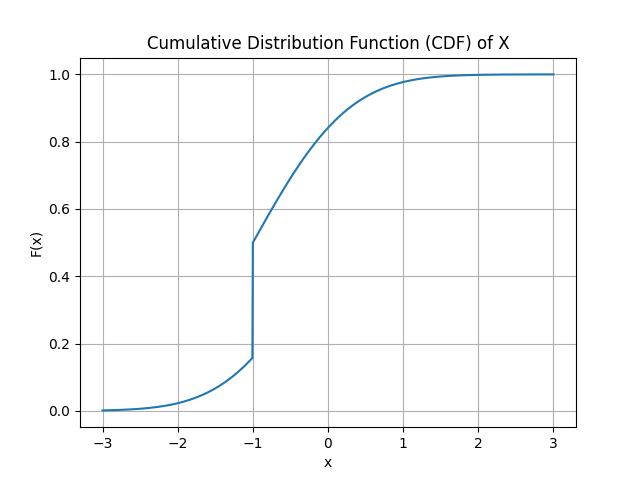
\includegraphics[width=\columnwidth]{/home/karthikeya/EE23010/15/figs/figure.png}
    \caption{}
    \label{fig:15st/2022}
\end{figure}
\newpage
\textbf{Box-Muller}\\
\textbf{STATEMENT}:
  Suppose U1 and U2 are independent samples chosen from the uniform distribution on the unit interval (0, 1). Let
  \begin{align}
  	Z_0 = R \cos(\Theta) =\sqrt{-2 \ln U_1} \cos(2 \pi U_2)\,
  \end{align}
   and
  \begin{align}
  	Z_1 = R \sin(\Theta) =\sqrt{-2 \ln U_1} \cos(2 \pi U_2)\, 
  \end{align}
  Then $Z_0$ and $Z_1$ are independent random variables with a standard normal distribution.
  So, now we will generate $Z_0$ using C Code as given below \\
\textbf{PROOF}:
  Let $X$ and $Y$ be independent standard normal variables 
  \begin{align}
  	X,Y \sim \mathcal{N}(0,1) \quad and \quad X\perp Y
  \end{align}
  The joint pdf of $X$ and $Y$ is given by 
  \begin{align}
  	f_{XY}(X,Y) &= f(x)f(y)\\
  	&= \frac{1}{\sqrt{2\pi}}e^{\frac{-x^2}{2}}.\frac{1}{\sqrt{2\pi}}e^{\frac{-y^2}{2}}\\
  	&= \frac{1}{2\pi}e^{\frac{-(x^2+y^2)}{2}}
  \end{align}
  The relationship between Cartesian coordinates $(x,y)$ and polar coordinates $(r,\theta)$ is as follows 
  \begin{align}
  	x=r\cos\theta \\
  	y=r\sin\theta
  \end{align}
  Change $f_{XY}(x,y)$ to polar coordinates :
  \begin{align}
  	f_{XY}(x,y) dxdy = f_{R\theta}(r,\theta) drd\theta
  \end{align}
  i.e.,
  \begin{align}
  	f_{R\theta}(r,\theta) = f_{XY}(x,y) \frac{dxdy}{drd\theta}
  	= f_{XY}(x,y) \mydet{\frac{\partial(x,y)}{\partial(r,\theta)}}
  \end{align}
  where J is the Jacobian 
  \begin{align}
  	J &= \mydet{\frac{\partial x}{\partial r} \,\, \frac{\partial x}{\partial \theta}\\\frac{\partial y}{\partial r} \,\, \frac{\partial y}{\partial \theta}}\\
  	&= \mydet{\cos\theta \,\, -r\sin\theta \\ \sin\theta \,\, r\cos\theta} = r
  \end{align}
  For $r\ge$ 0 and $\theta \in [0,2\pi)$, we have 
  \begin{align}
  	f_{R\theta}(r,\theta) drd\theta = \frac{1}{2\pi}e^{\frac{-(r^2)}{2}}rdrd\theta
  \end{align}
  Now we change the variable from $(r,\theta)$ to $(r^2,\theta)$;
  \begin{align}
  	rdr = \frac{1}{2}dr^2
  \end{align}
  Now it can be written as, 
  \begin{align}
  	f_{R\theta}(r,\theta)drd\theta &= f_{R^2\theta}(r^2,\theta)dr^2d\theta\\
  	&= \frac{1}{2\pi}e^{\frac{-(r^2)}{2}}\frac{1}{2}dr^2d\theta\\
  	&= \brak{\frac{1}{2}e^{\frac{-(r^2)}{2}}dr^2}\brak{\frac{1}{2}d\theta}\\
  	&= f_{R^2}(r^2)dr^2 f_{\theta}(\theta)d\theta
  \end{align}
  from the above equation, we can say that 
  \begin{align}
        R^2\perp\theta \,\, (i.e., R^2 \text{ and } \theta \text{ are independent})
  \end{align}
  Generate, $\theta \sim Unif(0,2\pi)$ 
  Generate, $V \sim Exp(\lambda = \frac{1}{2})$ (i.e., $V = R^2$) and compute 
  \begin{align}
        R=\sqrt{V}
  \end{align}
  Compute 
  \begin{align}
        X = R\cos\theta\\
        Y = R\sin\theta\\
  \end{align}
  where, $X,Y$ are i.i.d in $\sim \mathcal{N}(0,1)$
  Then  
  \begin{align}
        \theta &= 2\pi U_1\\
        V &= -2log(U_2)
  \end{align}
  We can prove $V = -2log(U_2)$ using the c.d.f definition of the exponential distribution\\
  Let $X$ be a random variable following an exponential distribution with rate parameter $\lambda = \frac{1}{2}$, denoted as $X \sim \text{Exp}\brak{\frac{1}{2}}$. The cumulative distribution function (CDF) of the exponential distribution is given by:
\begin{align}
F(x) &= 1 - e^{-\frac{x}{2}}
\end{align}
Now, suppose we have a random variable $U$ following a uniform distribution in the interval $[0, 1]$, denoted as $U \sim \text{U}(0, 1)$. The CDF of the uniform distribution is simply:
\begin{align}
F_U(u) &= u, \text{ for } 0 \leq u \leq 1
\end{align}
We can use the probability integral transform to express the exponential random variable $X$ in terms of the uniform random variable $U$:
\begin{align}
F(x) &= F_U(u) \\
1 - e^{-\frac{x}{2}} &= u
\end{align}
Now, solve for $x$:
\begin{align}
e^{-\frac{x}{2}} &= 1 - u \\
-\frac{x}{2} &= \ln(1 - u) \\
x &= -2 \ln(1 - u)
\end{align}
So, $X \sim -2 \ln(1 - U)$ for $U \sim \text{U}(0, 1)$. This expression represents the exponential random variable $X$ in terms of a uniform random variable $U$.\\
C and Python codes are given below :
  \lstinputlisting[language=C]{/home/karthikeya/EE23010/15/codes/rand.c}
  \lstinputlisting[language=Python]{/home/karthikeya/EE23010/15/codes/rand.py}
\begin{figure}[!ht]
  \centering
  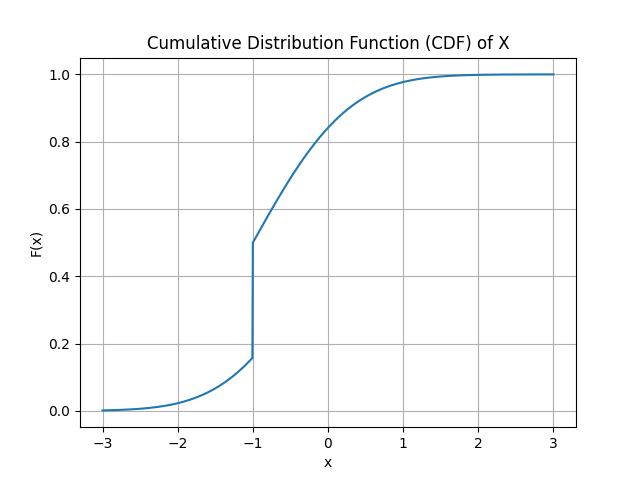
\includegraphics[width=\columnwidth]{/home/karthikeya/EE23010/15/figs/figure1.png}  % Replace 'image_filename' with your image file name
  \caption{Histogram plot of density of $Z_0$}
  \label{fig:your_label}
\end{figure}
\end{document}




















